\chapter{静态有向模型}
\label{chap:pgm-static-directed}

两个传感器的读数经常一起升高。可以直接建模第二个读数在第一个读数给定时的分布，也可以引入未观测的工作状态，让它共同影响两个读数。前一种方法拟合观测间的条件关系，后一种方法还要推断工作状态，并将它从联合分布中汇总掉。下面比较这两条建模路线怎样得到似然、回答缺失值查询，以及解释观测的相关性。

有向模型将联合分布写成局部条件概率的乘积，概率语义见第~\ref{chap:pgm-directed}章。本章选取静态模型，展开这些局部函数以及相应的推断和学习计算。这里的依赖没有沿真实时间演化的假设。一条记录记为$\bm x\in\mathbb R^d$或离散取值向量，训练数据为$\bm x_1,\ldots,\bm x_n$，待估参数统一记为$\bm\theta$；有类别标签时，用$Y$表示图中的类别节点。

先从全部建模变量都可观测的直接分解开始，再加入离散或连续的潜变量，分析求和与积分怎样形成观测分布。随后将多个记录按组组织，说明共享上层变量与每项选择成分的不同结构。潜变量的取值类型和记录间的共享方式可以同时变化，因此模型比较分别考察这两类选择，以及它们带来的计算和解释代价。

\section{直接模型}
\label{sec:pgm-static-directed-direct}

给定一条完整记录，就能在各节点读取父变量的取值，并计算局部条件概率的乘积。局部分布各自归一化后，这个乘积已经是合法的联合分布。缺失某些取值时，还需对它们求和或积分，计算规模随缺失模式改变。本节先限制属性的父集，再讨论用参数共享计算较大的条件分布。

\subsection{朴素贝叶斯与树增强模型}
\label{sec:pgm-static-directed-naive-tan}

训练数据同时记录设备类别与传感器读数时，可以先估计各类的读数分布，再据新读数计算类别后验。\term{朴素贝叶斯}（naive Bayes, NB）让类别成为所有属性的父节点，给定类别后，各属性共同独立。记$Y$有$K$类，先验为$\pi_k=p(Y=k)$，则
\begin{equation}
  \label{eq:pgm-static-directed-naive}
  p(y,\bm{x})=\pi_y\prod_{i=1}^{d}p(x_i\mid y),\qquad
  p(y\mid\bm{x})=
  \frac{\pi_y\prod_i p(x_i\mid y)}
       {\sum_{k=1}^{K}\pi_k\prod_i p(x_i\mid k)}.
\end{equation}
给定$Y$时的联合独立性，使各属性条件概率能够一起相乘；消去$Y$以后，共同类别仍可使属性相关。训练记录中的类别已知，最大似然估计分别计算类别比例和类内属性分布。预测新记录时，枚举$K$种类别，再将其权重归一化。此时$Y$是查询目标；模型主动引入的潜在状态与漏记的数据字段，则分别需要后面讨论的潜变量推断和缺失数据处理。

二值属性使用$a_{i,k}=p(X_i=1\mid Y=k)$。若类别$k$有$n_k>0$条记录，其中第$i$个属性为$1$的记录有$n_{i,k}^{+}$条，计数给出$\widehat\pi_k=n_k/n$、$\widehat a_{i,k}=n_{i,k}^{+}/n_k$。零计数会使某个条件概率为零，进而使完整记录的乘积为零；正的Dirichlet伪计数可以平滑这些表项。类别或父配置从未出现时，需要借助先验或其他约束估计其条件表。连续读数可采用类内高斯密度等函数，分布假设随之改变。

对两个类别和二值属性，在所有$a_{i,k}$及先验均严格位于$(0,1)$时，取伯努利似然的对数后验比，得到
\begin{equation}
  \label{eq:pgm-static-directed-naive-boundary}
  \begin{aligned}
  \log\frac{p(Y=1\mid\bm{x})}{p(Y=0\mid\bm{x})}
    &=b+\sum_{i=1}^{d}w_i x_i,\\
  b&=\log\frac{\pi_1}{\pi_0}
       +\sum_i\log\frac{1-a_{i,1}}{1-a_{i,0}},\\
  w_i&=\log\frac{a_{i,1}(1-a_{i,0})}
                       {a_{i,0}(1-a_{i,1})}.
  \end{aligned}
\end{equation}
这条线性评分来自伯努利条件概率的对数比。高斯属性若类间方差不同，对数比会带平方项；一般离散属性则以各状态的指示特征形成加性评分。NB先估计生成分布再得到系数，直接拟合分类损失则从类别预测目标估计系数，两者的学习方式不同。

\begin{example}[两个二值读数]
  \label{ex:pgm-static-directed-binary}
  另取一组人工参数，比较两个读数的直接分解与潜在解释。用$Y=1$表示异常工作状态，$X_1,X_2$表示二值读数，设
  \[
  \begin{gathered}
    p(Y=1)=0.1,\\
    p(X_1=1\mid Y=1)=0.8,\quad
    p(X_1=1\mid Y=0)=0.1,\\
    p(X_2=1\mid Y=1)=0.7,\quad
    p(X_2=1\mid Y=0)=0.2.
  \end{gathered}
  \]
  给定$Y$，两个读数独立生成。对观测$(X_1,X_2)=(1,1)$，两类权重为$0.1\times0.8\times0.7=0.056$与$0.9\times0.1\times0.2=0.018$，归一化得到
  \[
    p(Y=1\mid1,1)=\frac{0.056}{0.074}
      =\frac{28}{37}\approx0.7568.
  \]
  消去类别后，两个读数的边缘概率为$p(X_1=1)=0.17$、$p(X_2=1)=0.25$，联合概率$p(1,1)=0.074$却高于两边缘乘积$0.0425$。协方差为$0.0315$，显示共同类别引起的观测相关。
\end{example}

类内依赖也可能让两个读数重复提供同一信息。令第二个读数完全复制第一个，即$X_2=X_1$，并保持上述先验及$X_1$条件分布；两者为$1$时，正确后验为$0.08/(0.08+0.09)=8/17$。按独立属性重复相乘，却得到$0.064/(0.064+0.009)=64/73$，不仅改变按最大后验作出的类别判断，也放大对该判断的置信度。因此评价这项假设时，需要分别检查分类结果和后验概率。

为了表示类内依赖，可以在类别指向全部属性的结构上，再加入一棵属性树，得到\term{树增强朴素贝叶斯}（tree-augmented naive Bayes, TAN）。选属性$r$为根，将树边从根向外定向，非根属性$i$的属性父节点记为$t(i)$，联合分布为
\begin{equation}
  \label{eq:pgm-static-directed-tan}
  p(y,\bm{x})=
    p(y)p(x_r\mid y)
    \prod_{i\ne r}p(x_i\mid y,x_{t(i)}).
\end{equation}
每个非根属性增加一个属性父节点，给定类别后，各属性按树上的条件概率生成。图~\ref{fig:pgm-static-directed-classifiers}将这棵树与NB结构并列；新增边提供允许建模的依赖，若要解释为因果关系，还需额外的建模依据。

\begin{figure}[htbp]
  \centering
  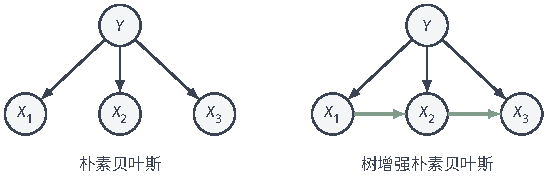
\includegraphics[width=92.650mm]{figures/06-probabilistic-graphical-models/04-models/tikz/pgm-static-directed-classifiers/figure.pdf}
  \caption{类别模型的两种属性结构。NB给定$Y$后各属性独立；TAN增加$X_1\to X_2\to X_3$，使右图的条件分布保留属性树上的依赖。训练时读入类别，预测时根据属性查询类别，观测状态随任务确定。}
  \label{fig:pgm-static-directed-classifiers}
\end{figure}

允许更大的父集，会增加需要估计的条件表。若属性$i$有$r_i$个状态，NB的自由参数为$(K-1)+K\sum_i(r_i-1)$；固定TAN属性树后，按父配置计数得到
\[
  (K-1)+K(r_r-1)
       +K\sum_{i\ne r}r_{t(i)}(r_i-1).
\]
两个类别和三个二值属性的自由参数由NB的$7$个增为TAN的$11$个，仍小于完整联合表所需参数，但新增父配置也需要数据支持。给定完整属性，两个模型枚举类别的评分均需$O(Kd)$次局部查询。二值TAN的对数评分还可含$x_i x_{t(i)}$项，因而能够表示属性间的交互。

对于完整离散数据，可以选择使训练似然最大的属性树。先用经验分布$\widehat p$计算给定类别的条件互信息
\[
  \widehat I(X_i;X_j\mid Y)=
  \sum_{y,x_i,x_j}\widehat p(y,x_i,x_j)
  \log\frac{\widehat p(x_i,x_j\mid y)}
                 {\widehat p(x_i\mid y)\widehat p(x_j\mid y)}.
\]
求和只计算正频数项，零频数项以连续延拓取$0$。将候选树上的条件表分别拟合为最大似然表，其平均训练对数似然为
\begin{equation}
  \label{eq:pgm-static-directed-tan-score}
  -\widehat H(Y)-\sum_i\widehat H(X_i\mid Y)
  +\sum_{\{i,j\}\in E_{\mathrm{T}}}
       \widehat I(X_i;X_j\mid Y),
\end{equation}
这里$\widehat H$是经验熵，$E_{\mathrm T}$是属性树的无向边集。每个非根属性的条件熵可写为$H(X_i\mid Y,X_j)=H(X_i\mid Y)-I(X_i;X_j\mid Y)$，根仍贡献$H(X_r\mid Y)$；将各项相加，便得到式中的熵项与树边互信息。熵项不随树改变，因此以条件互信息为边权，求最大生成树并任取根定向即可。这个最大似然结论针对观测完整、无结构惩罚和自由条件表的设定，其他约束需重新分析得分。

若$r_i\le r$，直接统计全部属性对需$O(nd^2)$次计数更新，遍历条件表求边权需$O(Kd^2r^2)$操作，稠密最大生成树需$O(d^2)$时间。NB只统计单属性，计数为$O(nd)$。TAN增加这部分工作以拟合类内依赖，树结构仍限制可表达的高阶相互作用；数据稀疏时，新增条件表和不稳定的树边可能增加估计误差。Friedman等给出了TAN及其算法，结构学习的一般得分推导见第~\ref{chap:pgm-structure-learning}章\scite{pgm-static-directed-friedman1997}

\subsection{自回归密度模型}
\label{sec:pgm-static-directed-autoregressive}

拟合观测的联合分布时，也可以依次为每个变量建立给定前面变量的条件分布。选定字段或像素的次序，把第$i$位以前的取值记为$\bm x_{<i}$。\term{自回归密度模型}（autoregressive density model）沿这个顺序计算条件概率，再相乘形成
\begin{equation}
  \label{eq:pgm-static-directed-ar}
  p_{\bm{\theta}}(\bm{x})
    =\prod_{i=1}^{d}p_{\bm{\theta}}(x_i\mid\bm{x}_{<i}).
\end{equation}
这种顺序规定预测前缀，例如表格字段排列或图像扫描顺序。第一个前缀$\bm x_{<1}$为空，因此第一项是边缘分布；各字段之间无需具有真实时间关系。

局部归一化保证式~\eqref{eq:pgm-static-directed-ar}的联合分布也归一化。离散变量先对$x_d$求和，最后一项变为$1$；依次消去$x_{d-1},\ldots,x_1$，最后留下$\sum_{x_1}p(x_1)=1$。连续变量使用非负可测、每个前缀下均归一化的条件密度，借助Tonelli定理依次积分，也得到总质量$1$。从某个联合分布恢复条件分布时，零概率前缀可补任意归一化条件分布，它与前缀零权重相乘后仍为零。归一化确定了概率合法性，拟合数据的质量还取决于所选条件函数。

链式法则允许任意联合分布沿任意变量排列分解。对二值变量使用完整条件表，仍需$1+2+\cdots+2^{d-1}=2^d-1$个自由参数。实际用有限宽度网络、有限感受野或高斯条件减少参数时，模型只保留这些局部函数可表达的分布。变量排列会改变待拟合的条件关系：一个方向的条件可能近似单峰，反向却可能出现多个峰，因此同样容量的函数在不同顺序下可产生不同误差。

消去例~\ref{ex:pgm-static-directed-binary}中的类别，得到两个读数的观测联合表
\[
  \begin{array}{ccccc}
    (x_1,x_2)&(0,0)&(0,1)&(1,0)&(1,1)\\
    p(x_1,x_2)&0.654&0.176&0.096&0.074
  \end{array}
\]
以$X_1$在前的顺序，将这张表改写为三个条件参数：
\[
  \begin{aligned}
    p(X_1=1)&=0.17,\\
    p(X_2=1\mid X_1=1)&=\frac{37}{85},\\
    p(X_2=1\mid X_1=0)&=\frac{88}{415}.
  \end{aligned}
\]
例如由$p(X_1=1)=0.17$和$p(X_2=1\mid X_1=1)=37/85$相乘，恢复$p(1,1)=0.074$。直接分解保留了整张读数联合表，用它能预测另一读数。若查询未观测工作状态$Y$，则还需要定义含$Y$的模型；观测表本身只给读数间的关系。

逐前缀条件表的大小随维数增长。\term{神经自回归分布估计器}（neural autoregressive distribution estimator, NADE）让不同前缀共用网络参数，以限制需要保存的参数量。对二值观测，宽度为$h$的单隐藏层条件函数为
\begin{equation}
  \label{eq:pgm-static-directed-nade}
  \begin{aligned}
    \bm{a}_i&=\bm{c}+\sum_{j<i}\bm{W}_{:,j}x_j,&
    \bm{h}_i&=\operatorname{sigmoid}(\bm{a}_i),\\
    p(X_i=1\mid\bm{x}_{<i})
      &=\operatorname{sigmoid}
        (b_i+\bm{V}_{i,:}\bm{h}_i).
  \end{aligned}
\end{equation}
其中$\bm W\in\mathbb R^{h\times d}$、$\bm V\in\mathbb R^{d\times h}$，$\bm c,\bm b$为偏置，$\operatorname{sigmoid}(u)=(1+\exp(-u))^{-1}$。前缀从$i$延长到$i+1$时，用$\bm a_{i+1}=\bm a_i+\bm W_{:,i}x_i$增量更新，成本为$O(h)$；配合每位的输出计算，完整记录评价需$O(dh)$操作。$\bm h_i$由已知前缀确定，可直接计算，无需作为随机潜变量积分。这个前缀复用方式构成NADE计算似然的基础\scite{larochelle2011}

也可以同时计算各条件，但限制每个输出能读取的输入。\term{掩码自编码分布估计器}（masked autoencoder for distribution estimation, MADE）将违反自回归顺序的连接置零。给输入$j$次序号$j$、隐藏单元$u$次序号$m(u)$，仅保留输入边$j\le m(u)$与输出边$m(u)<i$。深层隐藏边的次序号非递减，输出端仍要求严格小于$i$，故每条输入到输出的路径都满足$j<i$。这样同时算出的第$i$个条件只使用合法前缀。

图~\ref{fig:pgm-static-directed-mask}取三个输入和两个次序号分别为$1,2$的隐藏单元。以接收端为行、发送端为列，输入与输出掩码为
\[
  \bm{M}_{\mathrm{in}}=
  \begin{pmatrix}1&0&0\\1&1&0\end{pmatrix},\qquad
  \bm{M}_{\mathrm{out}}=
  \begin{pmatrix}0&0\\1&0\\1&1\end{pmatrix}.
\]
矩阵相乘得到$\left(\begin{smallmatrix}0&0&0\\1&0&0\\2&1&0\end{smallmatrix}\right)$，其非零项只在严格下三角，元素$2$计数两条合法路径。第一个条件输出仅用偏置，第三个输入只作为第三位似然的目标值，未进入任何条件参数。普通自编码器允许输出访问当前输入，可以通过复制完成重构；MADE用上述掩码约束，将重构形式转为合法的自回归密度计算\scite{pgm-static-directed-germain2015}

\begin{figure}[htbp]
  \centering
  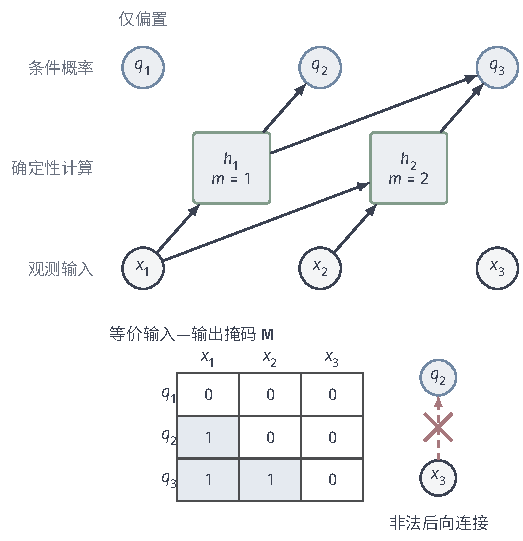
\includegraphics[width=88.554mm]{figures/06-probabilistic-graphical-models/04-models/tikz/pgm-static-directed-mask/figure.pdf}
  \caption{MADE掩码限定的条件依赖。隐藏方框进行确定性计算，输入与输出用圆框表示，$q_i=p(X_i=1\mid\bm x_{<i})$。下方输入—输出掩码的蓝色1标出允许读取的前缀，右侧$x_3\to q_2$展示违反顺序的连接；各隐藏单元的次序号共同保证输出只能读取此前的输入。}
  \label{fig:pgm-static-directed-mask}
\end{figure}

对图像，可用卷积共享不同位置的条件函数。\term{像素卷积自回归模型}（PixelCNN）按逐行扫描顺序，用掩码卷积读取当前像素上方和同行左侧的上下文。输入层排除当前目标值，后续层可读取当前位置已由合法前缀形成的隐藏表示。彩色图像还须规定像素内的通道顺序，例如红、绿、蓝，以使每个通道只访问此前通道。有限层数和卷积核限制可用感受野，模型虽归一化，却可能只利用部分前缀。原始论文同时介绍PixelCNN与PixelRNN，这里采用其中卷积掩码的依赖约束\scite{pgm-static-directed-oord2016}

每个输出层需定义当前变量的完整条件分布。二值变量使用伯努利参数，有$r$个状态的变量使用softmax归一化概率；原始PixelCNN对每通道的$256$个离散值采用后一种方式。连续条件可以输出均值$\mu_i(\bm x_{<i})$和正尺度$\sigma_i(\bm x_{<i})$来定义高斯密度，多峰条件则输出有限高斯混合的权重、均值和尺度。局部成分指示可被显式求和，因此混合参数化仍能计算这一条件似然。离散质量与连续密度使用不同的参考测度；将量化像素连续化时，还需给出量化区间积分或去量化方案。

完整训练记录提供每一位真实前缀，对这些条件分布的负对数似然求和，形成
\begin{equation}
  \label{eq:pgm-static-directed-ar-loss}
  L(\bm{\theta})=-\sum_{j=1}^{n}\sum_{i=1}^{d}
      \log p_{\bm{\theta}}
      (x_{j,i}\mid\bm{x}_{j,<i}).
\end{equation}
MADE和PixelCNN按固定网络深度前向计算，就能同时获得训练记录各位置的条件参数，再按式~\eqref{eq:pgm-static-directed-ar-loss}累加梯度，更新共享权重。传统NADE使用前缀递推，所有条件也共同决定共享参数的梯度。额外的跨位置计算需要保持相同的读取约束，例如将全部输入汇总后广播到每个输出，会重新引入未来或当前目标信息。

生成记录时，条件所需的前缀尚待抽样。先取$X_1$，再据其结果取$X_2$，沿顺序继续，完成祖先采样。具有完整顺序依赖的标量模型要作$d$轮相继决策，不同记录可以批处理，同一记录则按前缀推进。缓存减少各轮重复计算，但前后状态的依赖仍保留。NB在类别给定后各属性独立，可并行抽样；TAN可按属性树的层次并行，生成顺序因此取决于具体父集。

自回归分解提供可计算的完整似然和顺序采样。观测的是前缀时，余下部分可按原条件分布续写；若第一位缺失、后面的多位已观测，计算第一位的后验可能需要汇总一批变量。选择模型时，应分别评估完整密度、祖先采样和任意条件补全的成本。第~\ref{chap:pgm-generative}章将沿用这条直接似然路线，与其他神经生成构造比较。

\section{潜变量模型}
\label{sec:pgm-static-directed-latent}

聚类或压缩任务有时需要一个共同状态来解释多项读数，组间共享任务也需要表示记录背后的共同变化。为此可在观测外引入随机潜在坐标，再处理它们给定观测后的不确定性。\term{潜变量}（latent variable）指模型主动加入的未观测状态，漏记的字段则属于缺失数据，这一区别见第~\ref{sec:pgm-parameter-learning-definition}节。记潜在状态为$\bm z$，从它与观测的联合分布汇总得到
\begin{equation}
  \label{eq:pgm-static-directed-marginal}
  p_{\bm{\theta}}(\bm{x})=
  \begin{cases}
    \sum_{\bm{z}}p_{\bm{\theta}}(\bm{z})
          p_{\bm{\theta}}(\bm{x}\mid\bm{z}),
          &\text{离散潜变量},\\
    \int p_{\bm{\theta}}(\bm{z})
          p_{\bm{\theta}}(\bm{x}\mid\bm{z})\,d\bm{z},
          &\text{连续潜变量}.
  \end{cases}
\end{equation}
先验及各状态下的条件分布归一化，使观测分布的总质量为$1$。计算这个分布还要完成求和或积分，具体难度取决于潜变量和函数表示。仅由观测似然选择潜在解释时，也可能得到不同的等价分解；若要赋予它因果含义，需要更多依据。

\subsection{离散潜变量与有限混合}
\label{sec:pgm-static-directed-mixtures}

如果设备记录只含读数，工作状态可能由几个未标记的类别组成。\term{有限混合模型}（finite mixture model）先抽取成分，再用该成分的分布生成一条完整记录。成分$Z\in\{1,\ldots,K\}$具有权重$\pi_k\ge0$、$\sum_k\pi_k=1$，局部参数为$\bm\theta_k$，则
\begin{equation}
  \label{eq:pgm-static-directed-mixture}
  p(Z=k,\bm{x})=\pi_k p(\bm{x}\mid\bm{\theta}_k),
  \qquad
  p(\bm{x})=\sum_{k=1}^{K}\pi_kp(\bm{x}\mid\bm{\theta}_k).
\end{equation}
权重描述成分在总体中的比例，成分函数描述该状态下读数怎样变化。给定这些共享参数，每条记录独立抽取自己的$Z_j$，再生成观测。例~\ref{ex:pgm-static-directed-binary}若不记录类别，两个类内伯努利乘积就成为两成分混合；对类别求和后，仍得到前面的二元联合表。

共同成分怎样产生读数相关，可以把协方差分成类内和类间两部分。对具有有限二阶矩的两个属性，全协方差公式给出
\[
  \operatorname{Cov}(X_1,X_2)=
  \mathbb{E}\!\left[\operatorname{Cov}(X_1,X_2\mid Z)\right]
  +\operatorname{Cov}\!\left(
       \mathbb{E}[X_1\mid Z],\mathbb{E}[X_2\mid Z]\right).
\]
成分内部条件独立时，第一项为零，类间均值的共同变化仍可使第二项非零。前面二值读数的类间项为$0.1\times0.9\times(0.8-0.1)\times(0.7-0.2)=0.0315$，与联合表一致。若成分内部还有相关性，则保留第一项；有限混合本身并不规定成分内属性独立。

连续读数可以采用\term{高斯混合模型}（Gaussian mixture model, GMM）：$p(\bm x\mid Z=k)=\mathcal N(\bm x;\bm\mu_k,\bm\Sigma_k)$，各协方差正定。全协方差以$d(d+1)/2$个参数允许不同方向的相关和伸展；对角协方差以$d$个参数表示条件独立的属性；球形$\sigma_k^2\bm I$只估一个尺度。也可要求所有成分共享协方差，减少参数并让各成分具有同样形状。每个成分即使使用对角协方差，混合后的类间变化仍能形成非对角的总体协方差。

固定参数后，用每个成分的先验权重乘该记录的密度，再对$K$项归一化，就得到\term{责任度}（responsibility），即记录属于各成分的后验概率。对高斯成分，第$t$轮参数下写成
\begin{equation}
  \label{eq:pgm-static-directed-responsibility}
  r_{j,k}^{(t)}=
  \frac{\pi_k^{(t)}
      \mathcal{N}(\bm{x}_j;\bm{\mu}_k^{(t)},\bm{\Sigma}_k^{(t)})}
       {\sum_{\ell=1}^{K}\pi_\ell^{(t)}
      \mathcal{N}(\bm{x}_j;\bm{\mu}_\ell^{(t)},\bm{\Sigma}_\ell^{(t)})}.
\end{equation}
对前面的二值混合，观测$(1,1)$属于异常成分的责任度同样是$28/37$。标签未记录时，这些后验权重需要由当前参数推断，参数又要依据这些记录的归属来估计，两项计算因而交替进行。

EM在每轮先用旧参数计算式~\eqref{eq:pgm-static-directed-responsibility}中的责任度，再固定这些权重，优化新参数，通用推导见第~\ref{chap:pgm-parameter-learning}章。对高斯混合，需要最大化的期望完全数据对数似然为
\[
  \begin{aligned}
    Q={}&\sum_{j,k}r_{j,k}^{(t)}
       \left(\log\pi_k-\frac12\log|\bm{\Sigma}_k|\right)\\
       &-\frac12\sum_{j,k}r_{j,k}^{(t)}
         (\bm{x}_j-\bm{\mu}_k)^\top
          \bm{\Sigma}_k^{-1}(\bm{x}_j-\bm{\mu}_k)
       +\text{常数}.
  \end{aligned}
\]
在$\sum_k\pi_k=1$下对权重求驻点，得到加权样本比例；均值驻点为加权观测均值；将它代入协方差项，得到加权残差二阶矩。记有效样本数$N_k^{(t)}=\sum_jr_{j,k}^{(t)}$，当它为正且协方差更新保持正定时，三个更新为
\begin{equation}
  \label{eq:pgm-static-directed-gmm-em}
  \begin{aligned}
    \pi_k^{(t+1)}&=\frac{N_k^{(t)}}{n},\\
    \bm{\mu}_k^{(t+1)}
      &=\frac{\sum_jr_{j,k}^{(t)}\bm{x}_j}{N_k^{(t)}},\\
    \bm{\Sigma}_k^{(t+1)}
      &=\frac{1}{N_k^{(t)}}\sum_jr_{j,k}^{(t)}
       (\bm{x}_j-\bm{\mu}_k^{(t+1)})
       (\bm{x}_j-\bm{\mu}_k^{(t+1)})^\top.
  \end{aligned}
\end{equation}
协方差约束决定最后一步怎样汇总残差：对角模型取对角元素，球形模型取迹再除以$d$。这两种更新直接极大化各自的受约束目标，估计过程中始终使用相应的协方差形式。

\begin{example}[一轮可复核的高斯混合EM]
  \label{ex:pgm-static-directed-gmm-em}
  取一维人工记录$x_1=-1,x_2=1$，两个成分初始权重均为$1/2$、均值为$-1,1$、方差均为$1$。在$x_1$处，两成分的加权密度比为$1:\exp(-2)$，责任度矩阵为
  \[
    \bm{R}^{(0)}
      =\begin{pmatrix}a&1-a\\1-a&a\end{pmatrix},
    \qquad a=\frac{1}{1+\exp(-2)}\approx0.880797.
  \]
  两个成分的有效样本数各为$1$，所以新权重均仍为$1/2$；均值更新得到$\mu_1^{(1)}=1-2a\approx-0.761594$、$\mu_2^{(1)}=2a-1$。样本平方均为$1$，加权二阶矩也为$1$，减去新均值的平方得到
  \[
    (\sigma_1^2)^{(1)}=(\sigma_2^2)^{(1)}
      =1-(2a-1)^2\approx0.419974.
  \]
  责任度同时为两个成分保留正权重，两个新均值因此向中间移动；方差再围绕这些新均值估计。例子展示一次E步与M步的数值变化，尚未评价多轮优化的终点或新数据上的表现。
\end{example}

全协方差GMM先分解$K$个协方差矩阵，成本为$O(Kd^3)$，再计算$nK$个二次型及加权协方差统计，通常需$O(nKd^2)$操作。对角表示将统计成本降为$O(nKd)$。固定参数时，有限混合的似然与成分后验由可计算的$K$项得到，精确求和保持可行；学习还需求解非凸优化并选择成分数。计算责任度时可先求对数权重，减去最大值，再指数化归一化，以降低高维密度下溢的风险。

无约束GMM存在密度退化路径：把某成分均值放到一个训练点，将协方差趋于零，该点的密度趋于无穷；其余成分继续覆盖其他记录，训练似然便可没有有限最大值。继续迭代少量样本的例子也会面临这种边界。协方差特征值下界、适当先验或受约束估计可限制这类路径，但相应地改变学习目标；手工重置成分还需另行检查单调性。实际可从分散记录或聚类中心多次初始化，比较所得解；有效样本数近零时，按预定规则处理空成分。选择成分数时，再结合留出似然和应用任务，评估新增成分在训练数据以外的收益。

参数还具有\term{标签交换}（label switching）对称性。对任意两个成分，同时交换权重、均值和协方差，式~\eqref{eq:pgm-static-directed-mixture}给出的观测分布完全相同，编号本身无法由数据确定。置换得到的是同一预测分布的命名变化，另一个局部极值则可能给出不同预测。某些混合族在条件满足时可除置换外识别，但这个两成分、两二值属性例子有$5$个自由参数，观测表仅有$3$个自由度，通常还存在其他非唯一分解。解释成分或汇总对称后验时，应保留这种差异：不同编号的参数直接平均，可能破坏原本有用的预测表示。Murphy的教材讨论混合分布及其估计\scite{pgm-murphy2012}

\subsection{线性高斯潜变量模型}
\label{sec:pgm-static-directed-linear-gaussian}

多个读数也可能随连续的负载或振动强度共同变化。用$q<d$个潜在坐标表示这部分变化，剩余各维由独有噪声解释，就得到\term{因子分析}（factor analysis, FA）的线性高斯模型
\begin{equation}
  \label{eq:pgm-static-directed-fa}
  \begin{aligned}
    \bm{Z}&\sim\mathcal{N}(\bm{0},\bm{I}_q),\\
    \bm{X}&=\bm{\mu}+\bm{W}\bm{Z}+\bm{\varepsilon},\\
    \bm{\varepsilon}&\sim\mathcal{N}(\bm{0},\bm{\Psi}),\qquad
    \bm{\Psi}=\operatorname{diag}(\psi_1,\ldots,\psi_d),
    \quad\psi_i>0.
  \end{aligned}
\end{equation}
潜变量$\bm Z$与噪声$\bm\varepsilon$独立，$\bm\mu\in\mathbb R^d$是观测均值，载荷$\bm W\in\mathbb R^{d\times q}$的每列说明一个潜在坐标怎样同时影响各读数。给定所有潜在坐标，均值中的各因子贡献相加，观测只剩对角协方差的独立噪声。

线性变换保留高斯形式，独立的潜在贡献与噪声又使协方差相加，因此积分消去潜变量后得到
\begin{equation}
  \label{eq:pgm-static-directed-fa-marginal}
  \bm{X}\sim\mathcal{N}(\bm{\mu},\bm{C}),\qquad
  \bm{C}=\bm{W}\bm{W}^{\top}+\bm{\Psi}.
\end{equation}
共同变化$\bm W\bm W^\top$的秩至多为$q$，对角$\bm\Psi$记录各传感器独有的噪声。这个约束规定了相关性必须由共同因子解释。若让噪声协方差完全自由，噪声也能吸收观测相关，因子与噪声间的分配就更加不确定。

将残余噪声约束为$\bm\Psi=\sigma^2\bm I_d$，得到\term{概率主成分分析}（probabilistic principal component analysis, PPCA）。FA分别估计每维噪声，PPCA要求在当前坐标单位下各方向噪声同方差。改变特征单位会改变后一假设的含义，因此尺度选择需要与噪声模型一致。两种模型都提供潜在表示，同时给出这些坐标的后验不确定性。

给定观测，需要估计潜在坐标及其误差。令中心化读数$\bm y=\bm x-\bm\mu$，后验二次项系数$\bm M=\bm I_q+\bm W^\top\bm\Psi^{-1}\bm W$，先验与条件密度相乘后的$\bm z$项为
\[
  \begin{aligned}
    -2\log p(\bm{z}\mid\bm{x})
      &=\bm{z}^{\top}\bm{z}
       +(\bm{y}-\bm{W}\bm{z})^{\top}
          \bm{\Psi}^{-1}(\bm{y}-\bm{W}\bm{z})
       +\text{常数}\\
      &=\bm{z}^{\top}\bm{M}\bm{z}
       -2\bm{z}^{\top}\bm{W}^{\top}\bm{\Psi}^{-1}\bm{y}
       +\text{常数}.
  \end{aligned}
\]
正定噪声使$\bm M$正定。对上式配方，写成$(\bm z-\bm m)^\top\bm M(\bm z-\bm m)+\text{常数}$，读取高斯中心和精度，得到
\begin{equation}
  \label{eq:pgm-static-directed-fa-posterior}
  \begin{aligned}
    p(\bm{z}\mid\bm{x})&=\mathcal{N}(\bm{z};\bm{m},\bm{S}),\\
    \bm{S}&=\bm{M}^{-1},\qquad
    \bm{m}=\bm{S}\bm{W}^{\top}\bm{\Psi}^{-1}
                  (\bm{x}-\bm{\mu}).
  \end{aligned}
\end{equation}
后验均值表示给定读数的潜在坐标估计，后验协方差量化剩余不确定性。权重$\bm\Psi^{-1}$让噪声较小的测量在相同载荷下贡献较多精度，先验则提供单位精度，使证据较弱的坐标向零收缩。在固定参数、完整观测的条件下，协方差由$\bm M$决定，读数数值只改变后验均值。

对独立同分布的完整记录，FA和PPCA的均值最大似然估计都是样本均值，先以$\bm y_j=\bm x_j-\overline{\bm x}$中心化。E步用旧参数和式~\eqref{eq:pgm-static-directed-fa-posterior}得到$\bm m_j,\bm S$，并形成二阶矩$\bm T_j=\bm S+\bm m_j\bm m_j^\top=\mathbb E[\bm Z_j\bm Z_j^\top\mid\bm x_j]$。M步对期望加权残差目标中的载荷求导，得到
\[
  \bm{W}^{(t+1)}\sum_j\bm{T}_j
     =\sum_j\bm{y}_j\bm{m}_j^\top.
\]
这个矩阵方程右乘$\left(\sum_j\bm T_j\right)^{-1}$，可写出载荷更新。每项$\bm T_j$都包含正定$\bm S$，所以在正噪声与有限参数的当前迭代下，系数矩阵可逆。实际计算可直接求解矩阵方程，避免显式构造逆矩阵。

估计噪声时，还需把潜在坐标的后验方差计入残差。用$\bm W_+=\bm W^{(t+1)}$表示新载荷，期望残差协方差为
\begin{equation}
  \label{eq:pgm-static-directed-fa-residual}
  \begin{aligned}
    \bm{R}=\frac1n\sum_j\bigl[
      &(\bm{y}_j-\bm{W}_{+}\bm{m}_j)
       (\bm{y}_j-\bm{W}_{+}\bm{m}_j)^\top\\
      &+\bm{W}_{+}\bm{S}\bm{W}_{+}^\top
    \bigr].
  \end{aligned}
\end{equation}
FA逐维取$\psi_i^{(t+1)}=\bm R_{i,i}$，PPCA取共同方差$(\sigma^2)^{(t+1)}=\operatorname{tr}(\bm R)/d$。残差的第二项将潜变量后验方差映射到观测空间；若省掉它，噪声估计会偏小。解析E步和这项M步共同构成模型的EM迭代，单调性条件见第~\ref{chap:pgm-parameter-learning}章。噪声趋于零时，还需检查边界解和数值条件。

PPCA的最大似然载荷也可由样本协方差求得。令$\bm S_x=n^{-1}\sum_j\bm y_j\bm y_j^\top$，特征值按$\lambda_1\ge\cdots\ge\lambda_d$排列，前$q$个特征向量组成$\bm U_q$。当其余特征值的平均值为正时，解为
\begin{equation}
  \label{eq:pgm-static-directed-ppca-ml}
  \begin{aligned}
    \widehat{\sigma}^2
      &=\frac{1}{d-q}\sum_{i=q+1}^{d}\lambda_i,\\
    \widehat{\bm{W}}
      &=\bm{U}_q
       (\bm{\Lambda}_q-\widehat{\sigma}^2\bm{I}_q)^{1/2}
       \bm{R}_0,\qquad
       \bm{R}_0\bm{R}_0^\top=\bm{I}_q,
  \end{aligned}
\end{equation}
其中$\bm\Lambda_q=\operatorname{diag}(\lambda_1,\ldots,\lambda_q)$。负对数似然的协方差项为$\log|\bm C|+\operatorname{tr}(\bm C^{-1}\bm S_x)$：固定模型特征值，迹的重排不等式要求把最大的模型方差与最大的观测方差对齐。此后每个自由方向贡献$\log c_i+\lambda_i/c_i$，在$c_i=\lambda_i$处最小；其余$d-q$维共用$\sigma^2$，对这部分总和求导就得到剩余特征值的平均数。保留方向的重根会产生主轴选择的不唯一性；噪声估计为零则到达奇异边界，正定高斯密度的公式需重新处理。Tipping与Bishop给出了这个似然解及EM方法\scite{tipping1999}

为比较概率表示与几何投影，在保留的$\lambda_i>\widehat\sigma^2$方向，将潜变量后验均值映回观测空间，得到
\[
  \widehat{\bm{W}}\bm{m}
    =\bm{U}_q\operatorname{diag}
       \left(1-\frac{\widehat{\sigma}^2}{\lambda_i}\right)_{i=1}^{q}
       \bm{U}_q^\top\bm{y}.
\]
PCA把读数正交投影到所选子空间，PPCA还按信噪比缩小其中的坐标。固定满列秩载荷并令$\sigma^2$趋于零，均值重构的极限才是列空间上的正交投影；零噪声处的模型分布位于低维支持，已不是全维正密度。这样可由有噪声的后验重构联系降维几何，同时保留噪声条件的作用。

取人工样本协方差的特征值$5,2,1$，只保留一个因子。PPCA估计$\widehat\sigma^2=(2+1)/2=1.5$，可选$\widehat{\bm W}=\sqrt{3.5}\bm u_1$，得到模型协方差特征值$5,1.5,1.5$。后两方向被共同噪声方差合并，潜变量后验方差为$(1+3.5/1.5)^{-1}=0.3$。均值重构为$0.7\bm u_1\bm u_1^\top\bm y$，显示相对于PCA投影的收缩幅度。

某些传感器未读取时，潜在状态的不确定性随证据减少而变化。记观测索引$O\subseteq\{1,\ldots,d\}$，缺失索引为$U$，在式~\eqref{eq:pgm-static-directed-fa-posterior}中只保留$\bm W_{O,:}$、$\bm\Psi_{O,O}$及$\bm x_O-\bm\mu_O$，得到$\bm m_O,\bm S_O$。再利用独立残余噪声，把这些后验矩传播到缺失读数，得到
\begin{equation}
  \label{eq:pgm-static-directed-fa-missing}
  \begin{aligned}
    \mathbb{E}[\bm{X}_U\mid\bm{x}_O]
      &=\bm{\mu}_U+\bm{W}_{U,:}\bm{m}_O,\\
    \operatorname{Cov}(\bm{X}_U\mid\bm{x}_O)
      &=\bm{\Psi}_{U,U}
        +\bm{W}_{U,:}\bm{S}_O\bm{W}_{U,:}^\top.
  \end{aligned}
\end{equation}
缺失读数的预测方差包括自身噪声$\bm\Psi_{U,U}$，以及共同因子尚不确定带来的$\bm W_{U,:}\bm S_O\bm W_{U,:}^\top$。填入条件均值只保存一个估计值；后续使用填补数据时，还需处理这两项预测误差。

\begin{example}[两台传感器对一个连续因子的测量]
  \label{ex:pgm-static-directed-fa-missing}
  取$q=1,d=2$、$\bm\mu=\bm{0}$、$\bm W=(1,2)^\top$和$\bm\Psi=\operatorname{diag}(1,4)$作为人工模型，观测协方差为
  \[
    \bm{C}=\begin{pmatrix}2&2\\2&8\end{pmatrix}.
  \]
  完整读数$(2,4)$给出后验精度$1+1^2/1+2^2/4=3$、线性项$1\times2/1+2\times4/4=4$，所以$Z\mid(2,4)\sim\mathcal N(4/3,1/3)$。

  只保留$X_1=2$，后验精度变为$2$，得到$Z\mid X_1=2\sim\mathcal N(1,1/2)$。第二读数的预测均值为$2\times1=2$，方差为$4+2^2/2=6$。在观测空间直接条件化，也得到均值$(2/2)\times2=2$和方差$8-2^2/2=6$，两条计算路线一致。
\end{example}

载荷及坐标存在\term{旋转不唯一性}（rotational non-identifiability）。任意正交$\bm R_0$下，将载荷变为$\bm W\bm R_0$、坐标变为$\bm R_0^\top\bm Z$，潜在先验和观测协方差都保持原样。数据似然因而只约束相应分布，一维时也无法确定因子符号。为把某个因子命名为物理强度，需要额外约束、实验或领域信息；FA还可能有载荷和独有噪声的其他分解歧义。

对完整记录和对角噪声，形成$\bm M$需$O(dq^2)$操作，分解它需$O(q^3)$；复用相关矩阵后，各记录后验均值的计算为$O(dq)$。用Woodbury恒等式和行列式引理，也能以潜在空间矩阵计算观测似然：
\[
  \bm{C}^{-1}=\bm{\Psi}^{-1}
    -\bm{\Psi}^{-1}\bm{W}\bm{S}\bm{W}^{\top}\bm{\Psi}^{-1},
  \qquad |\bm{C}|=|\bm{\Psi}|\,|\bm{M}|,
\]
这两个恒等式使密度评价可避开$d\times d$稠密分解。完整数据的一轮EM通常为$O(ndq+nq^2+dq^2+q^3)$，噪声更新只计算残差协方差的对角元素。相同缺失模式可共用后验精度，不同模式需分别形成矩阵。缺失数据的E步还要计算缺失量的条件矩，均值更新也要利用这些矩。只对已观测数据最大化似然的适用条件，需结合第~\ref{chap:pgm-parameter-learning}章的缺失机制与可忽略性分析。

\subsection{层次结构与混合成员}
\label{sec:pgm-static-directed-hierarchy-membership}

同型号设备在不同工厂工作，各厂参数可能相似又各有偏差；同一文档也可能同时包含设备和维修等多个主题。这类任务需要进一步规定哪些未知量跨记录共享、哪些选择在记录内部变化。下面从共同参数的混合和因子模型，转向组级参数及组内多成分分配。

\term{层次模型}（hierarchical model）让各组参数来自一个共享的上层分布，以联系组间规律。\term{板表示法}（plate notation）用带索引的框标出节点与边的重复范围：组板内、样本板外的节点每组复制一次，两板内部的节点在每组的每个样本复制一次。给定索引后展开这些副本及连接，就得到联合分解的完整图。板框表示重复组织，概率因子仍由展开后的节点和父集决定。

例如组$g$的测量服从$X_{g,j}\mid\mu_g\sim\mathcal N(\mu_g,\sigma^2)$，组均值来自$\mu_g\sim\mathcal N(m_0,\tau^2)$。给定组均值，所有测量独立；给定上层参数，各组均值也独立。取已知$m_0$及正数$\sigma^2,\tau^2$，组内$n_g$条记录的均值为$\overline x_g$，配方得到
\begin{equation}
  \label{eq:pgm-static-directed-pooling}
  \begin{aligned}
    \mathbb{E}[\mu_g\mid\bm{x}_g]
      &=a_g\overline x_g+(1-a_g)m_0,\\
    a_g&=\frac{n_g\tau^2}{\sigma^2+n_g\tau^2},\\
    \operatorname{Var}(\mu_g\mid\bm{x}_g)
      &=\left(\tau^{-2}+n_g\sigma^{-2}\right)^{-1}.
  \end{aligned}
\end{equation}
权重$a_g$随组内样本数增加而增大，随测量噪声增加而减小，后验均值在本组平均值与共享中心$m_0$之间变化。这称为\term{部分汇聚}（partial pooling）：保留组间差异，同时用共同分布约束数据较少的组。取人工参数$m_0=0,\tau^2=1,\sigma^2=4,\overline x_g=3$，两条测量得到后验均值$1$，二十条测量得到$2.5$。两种收缩程度来自先验与测量精度的相对比例。

上式的共享分布固定已知时，本组后验只读取本组数据；其他组的新增记录不会改变它。若用全部组估计$m_0,\tau^2$，或为它们设先验再联合推断，各组便通过未知共享量交换信息。例如将$\mu_g$作为潜在组参数进行EM，E步求其后验矩，共同$\tau^2$下的M步将$m_0$更新为各组$\mathbb E[\mu_g\mid\mathcal D]$的平均。完全贝叶斯方法继续积分共享参数的不确定性。组级分布假设需要与组间规律相符，否则向同一中心收缩会引入偏差。

同一组中每个局部观测还可以选择自己的成分，这种结构称为\term{混合成员}（mixed membership）。一篇同时讨论设备和维修的文档，每个词分别选择主题，文档的主题比例控制这些选择；主题本身是词概率分布，其语义名称需由数据和应用解释。设文档$g=1,\ldots,G$有$N_g$个词，词表大小为$v$，词编号为$X_{g,j}\in\{1,\ldots,v\}$。主题词概率向量$\bm\beta_k$与文档主题比例$\bm\pi_g$各自非负、分量和为$1$。

\term{概率潜在语义分析}（probabilistic latent semantic analysis, pLSA）为每篇训练文档估计一个固定比例$\bm\pi_g$。给定文档编号，词位置$j$先从$\operatorname{Categorical}(\bm\pi_g)$抽主题$Z_{g,j}$，再从相应$\bm\beta_{Z_{g,j}}$抽词，得到
\begin{equation}
  \label{eq:pgm-static-directed-plsa}
  p(\bm{x}_g\mid\bm{\pi}_g,\bm{\beta}_{1:K})
    =\prod_{j=1}^{N_g}
       \sum_{k=1}^{K}\pi_{g,k}\beta_{k,x_{g,j}}.
\end{equation}
$\operatorname{Categorical}$给出类别抽样概率，$\beta_{k,a}$是主题$k$产生词$a$的概率。给定固定比例与主题参数，不同词各有自己的主题后验，权重正比于$\pi_{g,k}\beta_{k,x_{g,j}}$，各位置的后验独立。EM用这些责任度更新文档比例为平均主题责任度，再按全语料加权词频更新主题分布。相同词可合并为词频以复用计算。Hofmann介绍了pLSA的混合分解与EM估计\scite{pgm-static-directed-hofmann1999}

pLSA的文档比例一共包含$G(K-1)$个自由参数，随训练文档数增长。遇到新文档，可固定已学主题，再由新词拟合一组比例，称为折入估计。这个步骤扩展了参数表，但原模型没有描述新比例的随机来源；需要组级生成时，就要进一步为比例定义分布。

\term{潜在狄利克雷分配}（latent Dirichlet allocation, LDA）为每篇文档的比例设置先验，使新文档也有相同的生成步骤。
比例先验采用Dirichlet分布（参考\BookSectionRef{sec:probability-common-distributions}{第一卷“数学准备”的常见分布模型小节}）。
记$\bm\pi_g\sim\operatorname{Dirichlet}(\bm\alpha)$，各$\alpha_k>0$，总质量为$\alpha_0=\sum_k\alpha_k$。
先抽文档比例，再逐词抽取主题和词值。
给定主题词分布，其联合分布及对比例、主题汇总后的观测分布为
\begin{equation}
  \label{eq:pgm-static-directed-lda}
  \begin{aligned}
    p(\bm{\pi}_g,\bm{z}_g,\bm{x}_g\mid
          \bm{\alpha},\bm{\beta}_{1:K})
      &=p(\bm{\pi}_g\mid\bm{\alpha})
         \prod_j\pi_{g,z_{g,j}}\beta_{z_{g,j},x_{g,j}},\\
    p(\bm{x}_g\mid\bm{\alpha},\bm{\beta}_{1:K})
      &=\int p(\bm{\pi}_g\mid\bm{\alpha})
          \prod_j\left(\sum_k
              \pi_{g,k}\beta_{k,x_{g,j}}\right)d\bm{\pi}_g.
  \end{aligned}
\end{equation}
这里固定文档长度，只建模其中的词。各文档共用$\bm\alpha$和主题分布，新文档的比例按先验产生，再根据词进行后验推断。于是模型给出了固定长度下的新文档生成分布，词序或语法还需别的结构描述。

给定$\bm\pi_g$，各位置的词独立同分布；积分掉这个共同随机比例后，位置间一般相关，但任意词序排列仍有相同概率，即词袋的可交换性。若把样本改为词计数向量，还需乘相应的多项式计数系数。LDA由此加入了pLSA所缺的文档级比例先验，同时需要处理比例积分；原始论文给出模型、变分推断和经验贝叶斯学习\scite{blei2003}

\begin{example}[固定比例、随机比例与整组单一主题]
  \label{ex:pgm-static-directed-lda-two-words}
  用两词词表$\{a,b\}$及主题$\bm\beta_1=(0.8,0.2)$、$\bm\beta_2=(0.2,0.8)$比较三种共享方式。取LDA先验$\bm\alpha=(1,1)$，则$\pi_{g,1}=u$均匀分布于$[0,1]$，$\pi_{g,2}=1-u$。给定$u$，词$a$的概率为$0.2+0.6u$，边缘为$1/2$；两词均为$a$时需要对同一个$u$积分，得到
  \[
    p(a,a)=\int_0^1(0.2+0.6u)^2\,du
      =0.04+0.12+0.12=0.28.
  \]
  固定比例$(1/2,1/2)$时，式~\eqref{eq:pgm-static-directed-plsa}给出$0.5^2=0.25$；整篇仅选一个主题时，概率为$(0.8^2+0.2^2)/2=0.34$。三种模型的单词边缘均为$1/2$，但共享方式导致双词联合概率不同。

  在LDA中，四种主题配置$(1,1),(1,2),(2,1),(2,2)$与$(a,a)$的联合概率为$16/75,2/75,2/75,1/75$。第一项由$\int_0^1u^2\,du\times0.8^2$得到，第二项由$\int_0^1u(1-u)\,du\times0.8\times0.2$得到。将四项归一化，后验配置权重为$16/21,2/21,2/21,1/21$，按各配置的比例后验组合，形成
  \[
    \begin{aligned}
      p(\bm{\pi}_g\mid a,a)
        ={}&\frac{16}{21}\operatorname{Dirichlet}(3,1)
           +\frac{4}{21}\operatorname{Dirichlet}(2,2)\\
           &+\frac{1}{21}\operatorname{Dirichlet}(1,3).
    \end{aligned}
  \]
  混合后验的均值为$\mathbb E[\pi_{g,1}\mid a,a]=19/28$，下一词为$a$的概率为$0.2+0.6\times19/28=17/28$。未知主题使比例后验成为多个Dirichlet分布的混合，各项对应不同的主题计数。
\end{example}

若每个词的主题都已知，计数$n_{g,k}$与先验共轭，直接给出$\bm\pi_g\mid\bm z_g\sim\operatorname{Dirichlet}(\bm\alpha+\bm n_g)$。只观测词时，这个后验需要按未知主题配置加权；长度$N_g$的文档有$K^{N_g}$种配置，枚举很快超出计算预算。下面用近似推断或单点采样处理这个配置空间，同时保留比例的不确定性。

全局主题也可设先验$\bm\beta_k\sim\operatorname{Dirichlet}(\bm\eta)$、$\eta_a>0$，如图~\ref{fig:pgm-static-directed-plates}所示。各文档共用$\bm\beta_k$，各词共用本篇的$\bm\pi_g$，主题分配$Z_{g,j}$则逐词取值。这些不同共享层级同时容纳连续比例与离散分配。

\begin{figure}[htbp]
  \centering
  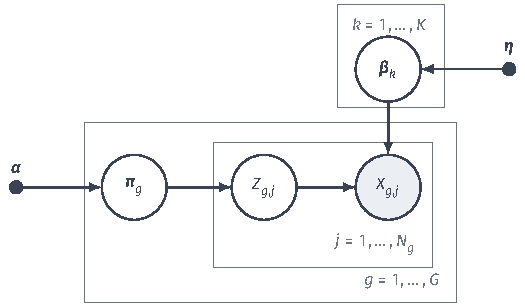
\includegraphics[width=88.935mm]{figures/06-probabilistic-graphical-models/04-models/tikz/pgm-static-directed-plates/figure.pdf}
  \caption{带全局主题先验的LDA重复结构。空心圆表示随机潜在量，填色圆表示观测词，实点表示给定超参数。文档板内每篇有一个$\bm\pi_g$，词板内每词有一组主题分配和观测；$K$个$\bm\beta_k$跨全部文档共享，词节点根据$Z_{g,j}$读取其中一个主题分布。}
  \label{fig:pgm-static-directed-plates}
\end{figure}

先固定$\bm\beta_{1:K}$，用平均场$q(\bm\pi_g)\prod_jq(Z_{g,j})$近似同篇文档的联合后验。选择$q(\bm\pi_g)=\operatorname{Dirichlet}(\bm\gamma_g)$和$q(Z_{g,j}=k)=\rho_{g,j,k}$，交替优化比例因子与主题因子，得到坐标更新
\begin{equation}
  \label{eq:pgm-static-directed-lda-vi}
  \begin{aligned}
    \rho_{g,j,k}&\propto
      \beta_{k,x_{g,j}}
       \exp\!\left\{\psi(\gamma_{g,k})
                   -\psi\!\left(\sum_\ell\gamma_{g,\ell}\right)\right\},\\
    \gamma_{g,k}&=\alpha_k+\sum_j\rho_{g,j,k}.
  \end{aligned}
\end{equation}
函数$\psi(u)=d\log\Gamma(u)/du$为digamma，指数中的项是$q$下的$\log\pi_{g,k}$期望。局部参数$\bm\phi_g$由$\bm\gamma_g,\bm\rho_g$组成，每个词先归一化$\rho$，再交替更新两式。这是第~\ref{chap:pgm-variational}章的坐标上升在LDA中的应用，得到指定变分族内的近似。固定全局参数时，一轮稠密更新通常需$O(K\sum_gN_g)$操作。

在主题词分布也有Dirichlet先验的设定下，先积分掉$\bm\pi_g$和$\bm\beta_k$，再使用第~\ref{chap:pgm-sampling}章的Gibbs方法更新一个词的主题。排除当前位置后，文档主题计数记为$n_{g,k}^{-}$，全语料主题词计数为$c_{k,a}^{-}$，并记$c_{k,\cdot}^{-}=\sum_a c_{k,a}^{-}$、$\eta_0=\sum_a\eta_a$，单点条件为
\begin{equation}
  \label{eq:pgm-static-directed-lda-gibbs}
  p(Z_{g,j}=k\mid\text{其余分配},\mathcal{D})
     \propto (n_{g,k}^{-}+\alpha_k)
        \frac{c_{k,x_{g,j}}^{-}+\eta_{x_{g,j}}}
             {c_{k,\cdot}^{-}+\eta_0}.
\end{equation}
文档主题计数给出第一项，主题词计数给出第二项，二者是相应共轭后验的预测权重；文档分母与$k$无关，已经抵消。相乘并归一化，得到精确的单点条件分布。有限轮Gibbs样本构成的整体后验估计仍需考虑抽样误差和混合速度。

将主题词分布作为点参数时，变分EM先固定当前主题，求各文档的局部近似，再用$\rho$加权的全语料词频更新主题概率。比例先验参数$\bm\alpha$的目标包含$\log\Gamma(\alpha_0)-\sum_k\log\Gamma(\alpha_k)$及各文档$\mathbb E_q[\log\pi_{g,k}]$，在正值约束下数值优化。使用变分期望后，迭代分析针对变分目标，观测似然的变化还需另行检查。若主题参数也作为随机量，就更新其后验或变分因子；第~\ref{chap:pgm-parameter-learning}章分别讨论这些学习目标。

在对称主题先验下，同时置换主题编号和比例坐标，观测分布保持不变。非对称先验可约束部分编号，有限语料中的主题词分布仍可能有其他歧义；相近主题、短文档或过大的主题数会加剧不稳定性。词袋和比例先验各自限制了词序及组间变化，解释主题含义时，需要同时评价这些假设和分解的稳定性。

有限混合和主题模型先给定候选成分数$K$。
\term{狄利克雷过程混合}（Dirichlet process mixture, DPM）为混合测度设置随机先验，让有限数据中的占用成分数参与推断。
在标准Borel成分参数空间上，记这个随机概率测度为$G\sim\operatorname{DP}(c,H)$。
其中$c>0$控制总质量，$H$是基概率测度；它们分别对应卷一的$\alpha$和$G_0$。
本节采用$c,H$，以区分主题比例先验的参数。
Dirichlet过程由全部有限分割上的Dirichlet规律刻画，
相应定义见\BookSectionRef{sec:rv-random-generation}{第一卷“数学准备”的随机概率测度与Dirichlet过程小节}。

折棒构造提供可供混合建模使用的可数表示。
独立抽取$v_k\sim\operatorname{Beta}(1,c)$与$\bm\xi_k\sim H$，依次给剩余质量分配比例$v_k$，令
\[
  w_k=v_k\prod_{\ell<k}(1-v_\ell),\qquad
  G=\sum_{k=1}^{\infty}w_k\delta_{\bm{\xi}_k}.
\]
其中$\delta_{\bm\xi_k}$是原子处的点质量；折棒构造定理保证这个$G$具有上述有限分割规律。
权重和为$1$给出概率测度的归一化，Dirichlet过程分布还依赖这些分割规律。
Teh等的论述介绍了相应构造及其用于层次共享的方式\scite{pgm-static-directed-teh2006}
给定$G$，各记录独立抽取$\bm\zeta_j\mid G\sim G$，再按$\bm X_j\mid\bm\zeta_j\sim p(\cdot\mid\bm\zeta_j)$生成读数。
记录重复抽到一个原子，就使用同一成分参数；成分分布仍可连续。

给定$n$个潜在成分参数，在任意有限分割上，用各单元的计数更新Dirichlet先验。
把这些相容的分割更新合在一起，得到随机测度的后验
\[
  G\mid\bm\zeta_{1:n}\sim\operatorname{DP}
    \left(c+n,\frac{cH+\sum_{j=1}^n\delta_{\bm\zeta_j}}{c+n}\right).
\]
下一条记录的成分参数预测分布由这个后验的均值给出。

取无原子的$H$并积分掉$G$，前$n$个潜在参数中占用成分$k$的计数为$n_k$，下一条复用它的概率为$n_k/(n+c)$，新抽成分的总概率为$c/(n+c)$。已有计数$(3,1)$、$c=1$时，三个选择分别为$0.6,0.2,0.2$。若该条读数也已给定，还需乘各已有成分和基准测度下的预测密度，再归一化。有限$n$至多占用$n$个成分，第$j$次增加成分的先验概率为$c/(c+j-1)$，所以占用数的先验期望是这些概率之和$\sum_{j=1}^n c/(c+j-1)$。可数先验放宽候选容量，实际推断处理当前占用或截断的候选成分，恢复真实有限类别数还需要其他条件。

多个组需要共享成分时，还要让它们使用相同原子。从同一个无原子$H$分别抽取独立Dirichlet过程，各组的原子几乎必然不同。\term{层次狄利克雷过程}（hierarchical Dirichlet process, HDP）先抽离散的随机基准，再由它生成组测度：
\begin{equation}
  \label{eq:pgm-static-directed-hdp}
  G_0\sim\operatorname{DP}(\gamma,H),\qquad
  G_g\mid G_0\sim\operatorname{DP}(c,G_0).
\end{equation}
$G_0$几乎必然离散，所以各$G_g$共用同一可数原子集合，同时分别具有组级权重。在主题模型中，这些原子是词分布，每篇文档按自己的权重逐词选择共享主题。一个模型因此同时具有层次共享、混合成员及非固定成分数；这些属性描述不同的组织方式。Teh等进一步说明DP构造和HDP共享原子的机制\scite{pgm-static-directed-teh2006}

DPM和HDP将成分数量选择与分配、权重、超参数一同纳入推断。截断变分用有限候选近似可数模型，需要检查截断误差；采样调整占用成分，需要检查链的混合。HDP还要共同处理组级成分和全局原子的关系，独立拟合各组有限混合无法完成这项共享推断。浓度参数影响分组倾向，需结合超参数估计和预测检验使用。输出时可报告预测、占用数及组间共享的不确定性，原子编号本身仍只承担命名。

\section{模型比较}
\label{sec:pgm-static-directed-comparison}

先固定查询和被积分的随机量，才能比较计算。在表~\ref{tab:pgm-static-directed-comparison}中，给定所选全局参数或超参数，按各模型的设定汇总随机潜在量，得到观测似然$p(\bm x)$；用点估计固定的参数不再积分。NB和TAN的完整训练记录为$(y,\bm x)$，类别预测时则对$Y$归一化。独立性、共享和非唯一性另列，便于分析同一种查询在不同结构中需要完成哪些工作。

\begin{table*}[htbp]
  \centering
  \small
  \begin{tabularx}{\linewidth}{@{}
    >{\raggedright\arraybackslash}p{28mm}
    >{\raggedright\arraybackslash}p{30mm}
    >{\raggedright\arraybackslash}p{27mm}
    >{\raggedright\arraybackslash}p{30mm}
    >{\raggedright\arraybackslash}X@{}}
    \toprule
    模型与潜在量 & 独立性与共享 & 观测似然 & 局部后验 & 非唯一性与主要代价\\
    \midrule
    NB／TAN：训练时无潜变量 &
    类内独立／类内树；参数跨样本共享 &
    完整记录直接乘积 &
    类别后验枚举$K$项 &
    支持不足的条件表不确定；TAN还需选择树\\
    自回归：无随机潜变量 &
    顺序父集；条件网络可共享参数 &
    条件密度直接乘积 &
    前缀续写直接；任意补全未必易算 &
    网络参数可不唯一；优化、顺序选择与串行生成\\
    有限混合：离散分配 &
    样本在固定参数下独立；类内结构由成分决定 &
    $K$项有限和 &
    成分责任度精确 &
    标签交换、冗余成分；局部极值与退化\\
    FA／PPCA：连续因子 &
    给定因子后观测独立；共享载荷 &
    解析高斯密度 &
    解析高斯后验与缺失预测 &
    旋转及可能的额外分解歧义；维数与噪声假设\\
    LDA：连续比例与离散主题 &
    组级比例、全局主题；组内条件独立 &
    需积分比例，通常近似 &
    联合后验通常近似，局部条件可解析 &
    主题置换与重叠；局部推断和全局学习交替\\
    DPM／HDP：分配与随机测度 &
    可数候选成分；HDP跨组共享原子 &
    对未知随机量积分通常需近似 &
    采样或截断变分 &
    成分编号不唯一；占用数、超参数与近似误差\\
    \bottomrule
  \end{tabularx}
  \caption{静态有向模型在给定参数或超参数下的计算。表中的精确结果指相应有限求和、解析积分或局部条件；学习目标、参数不确定性及潜在解释另按各模型分析。}
  \label{tab:pgm-static-directed-comparison}
\end{table*}

直接模型以局部条件拟合观测联合分布。NB用类内独立减少待估参数，TAN增加树边及结构搜索，神经自回归则用非线性条件与参数共享扩大可表达的关系。完整记录可直接计算局部乘积，祖先生成和缺失查询还需按各自依赖进行。潜变量路线也可能保留精确计算：有限混合显式汇总$K$项，线性高斯模型解析积分，同时给出似然和局部后验。

共享随机量会联系不同位置的推断。pLSA固定文档比例时，逐词做有限求和；LDA积分共同的文档比例后，主题分配需要一起解释这些词。全局主题再带先验时，不同文档也相互联系，HDP还需要推断共享的占用成分。这些联系决定了联合后验的规模，除各变量的状态数外，还需考察它们共同读取哪些数据。

也可以组合上述属性。混合因子分析为每个离散成分配置连续因子，成分内积分后仍是低秩加对角协方差的高斯，所以成分责任度和因子后验可解析计算。自回归条件可采用有限混合，组级载荷可设置层次先验。因此离散或连续、线性高斯或非线性、组间共享或独立、逐项生成或联合生成，分别描述模型的一项选择。

观测分布估计准确时，潜在解释仍可能受对称性约束：网络权重可有多种表示，成分可交换编号，因子可旋转方向。选择模型时，可先用留出数据评价预测，再按目的检查所需输出；解释结构需要报告对称性及稳定性，补全任务则需要评价条件预测和误差范围。似然计算、预测表现和潜在语义各有相应的核验对象。

\section{本章小结}
\label{sec:pgm-static-directed-summary}

静态有向分解把局部条件组合成联合分布。全部变量可观测时直接读取乘积，引入潜在状态后则先汇总它们，得到观测分布。两个传感器的同一联合表可用自回归条件或隐藏类别的混合表示，前者给出读数预测次序，后者加入需要另行验证的工作状态解释。

有限混合用责任度与成分参数交替学习，固定参数的局部后验仍可精确求得。线性高斯积分把观测协方差、降维和缺失预测联系起来；共享随机量与混合成员联系多个记录或组的推断，联合计算可能需要近似。取值类型与共享方式可以组合使用，标签置换、因子旋转和其他分解歧义则限制了潜在坐标的唯一解释。

判断新模型时，可以从联合归一化、查询待消变量、共享范围和估计的边界条件逐项展开。第~\ref{chap:pgm-energy-models}章接着采用对称相互作用，比较联合归一化与输出条件归一化。第~\ref{chap:pgm-generative}章再以自回归和高斯潜变量为参照，讨论神经网络如何参数化更灵活的密度，以及相应概率计算的代价。

\paragraph{扩展阅读}
Bishop的PRML用混合、潜变量及变分学习展开静态模型，Koller与Friedman从局部条件结构讨论共同的推断与学习方法。可沿同一图的作用域比较不同局部分布，检查哪些求和或积分仍有解析形式，哪些学习目标需要近似后验\scite{bishop2006,pgm-koller2009}
